\chapter{Treplica Reconfigurável}\label{cap2}

Cobiçamos para Treplica um mecanismo de autogestão capaz de realizar autointegração de
réplicas sem intervenção humana, inteligente o suficiente para detectar oscilação na
demanda e reagir a elas, proporcionando assim maior eficiência na utilização de recursos
físicos. Projetar mecanismos autônomos sintonizados para reagir rapidamente às mudanças no
sistema é um assunto atual e relevante para pesquisa.

O primeiro passo para suportar tal anseio é dado nesse trabalho, que tem como objetivo
transformar Treplica em uma biblioteca reconfigurável. O problema de reconfiguração é
complexo, principalmente na presença de falhas e assincronia. Sua resolução é obtida
basicamente a partir de duas maneiras: (1) Abordagem baseada em transições de visões do
conjunto de réplicas participantes (e corretas) \cite{birman87a, birman87b}; (2)
Definição, via consenso, de uma nova configuração a partir da construção de uma barreira
que, quando alcançada pelas réplicas, faz com que elas abandonem a configuração vigente e
ingressem na nova configuração definida (caso elas façam parte dela) \cite{lamport10}.

Para o processo de reconfiguração, identificamos a necessidade de um mecanismo eficiente
capaz de transferir estado entre réplicas. Treplica ainda não possui tal mecanismo capaz
de oferecer um poder de manobra para adição de novas réplicas e recuperação de falhas.
Estamos preocupados com o impacto inerente para implantar uma nova réplica em um
aglomerado em tempo de execução. Se perceptível tal impacto dificulta a viabilidade das
técnicas de autogestão, porque dependendo do cenário, adicionar uma nova réplica pode
comprometer o desempenho de um sistema sobrecarregado \cite{vilaca09}.

Neste capítulo apresentamos os principais componentes de Treplicas que serão de
fundamental importância para compreender as alterações propostas na biblioteca, que tambem
estao contemplandas nesse capitulo. Comecamos com uma \autoref{sec:visao_arquitetural},
nessa secao apresentamos os componentes de suporte fundamentais para arquitetura de
Trepica e examinamos detalhadamente os componentes utilizados para construção do algoritmo
Paxos. Em seguida, na \autoref{sec:alteracoes_propostas} apresentamos minunciosamente as
alterações e os novos componentes propostos para Treplica.


\section{Visão arquitetural de Treplica}\label{sec:visao_arquitetural}

A arquitetura de Treplica eh baseada em uma fila persistente assíncrona
\autoref{fig:paxos_persistent_queue}, sua implementacao segue muito de perto a
decomposicao modular de Paxos especificada por \citeonlie{lamport10}. A fila é composta
por classes internas da biblioteca que resprensentam a funcionalidade dos quatro agentes
de Paxos:

\begin{figure}[ht]
  \centering
  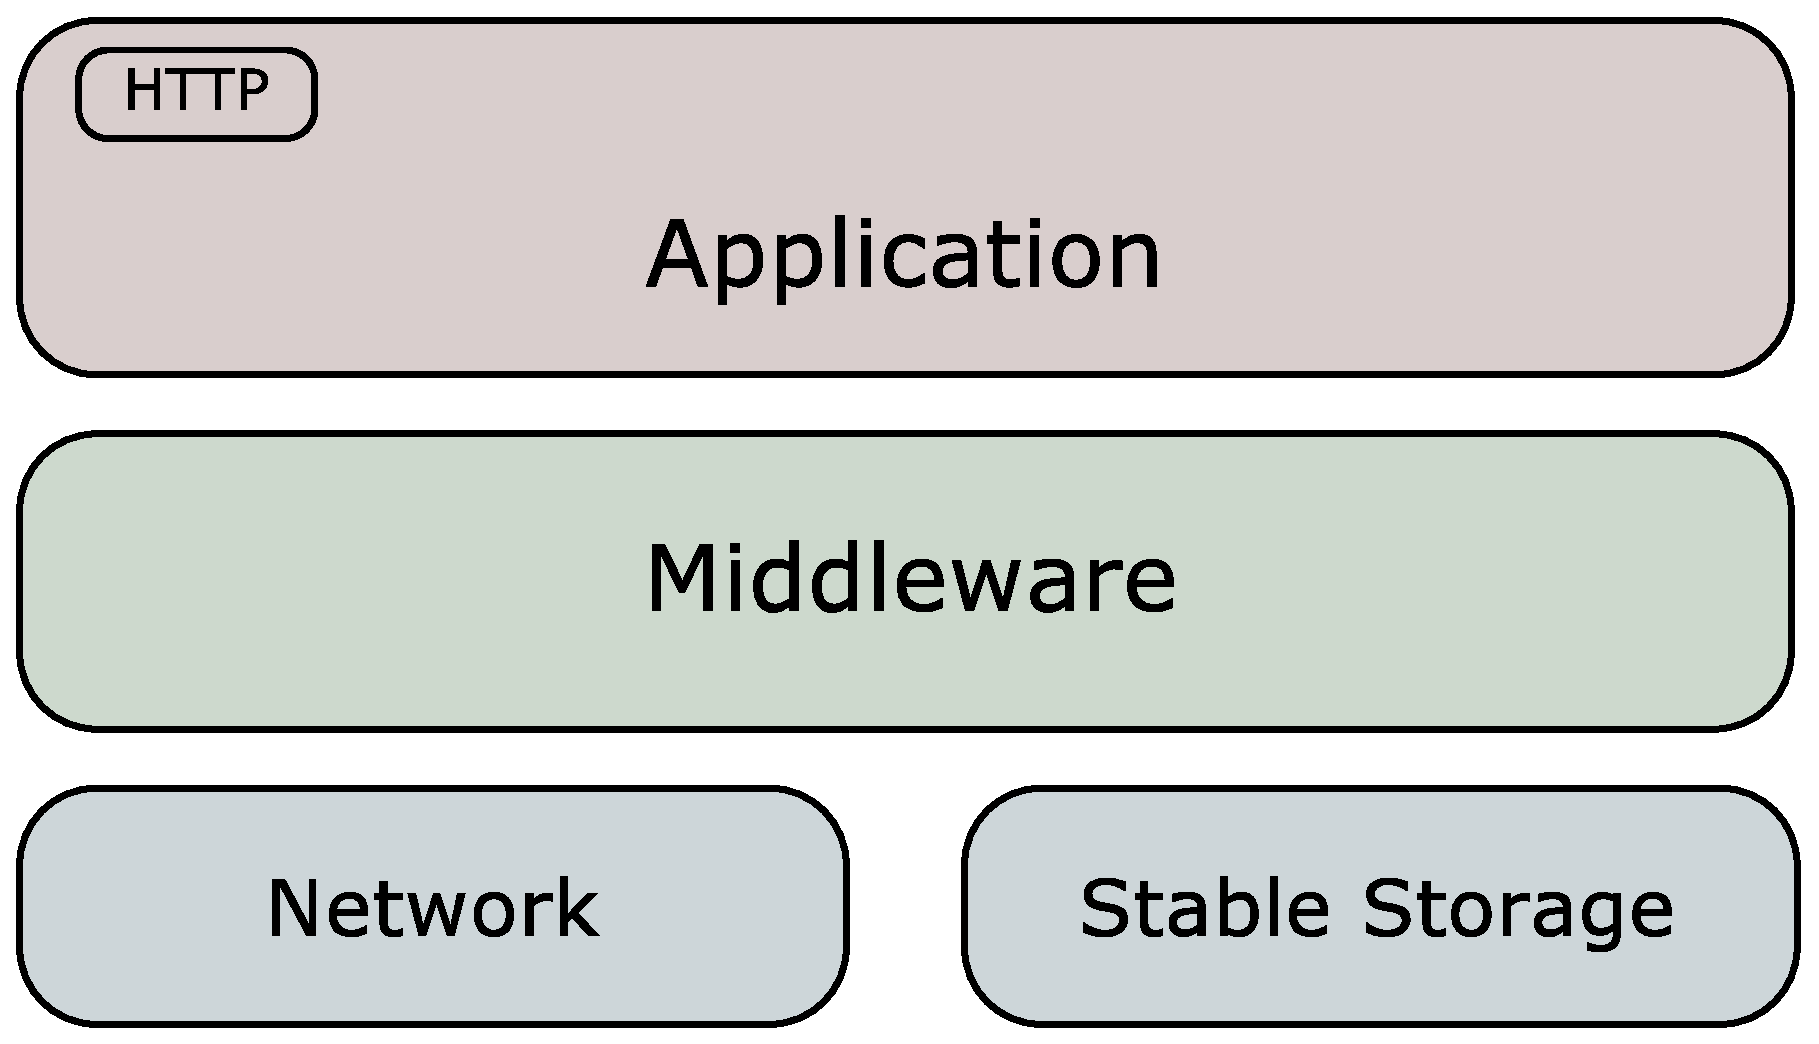
\includegraphics[width=12cm]{conteudo/capitulos/figuras/block-simple.eps}
  \caption{Paxos Persistent Queue}
  \label{fig:paxos_persistent_queue}
\end{figure

\begin{itemize}
  \item \classname{Learner} combina os agentes proponentes e aprendiz em uma unica classe
    resposavel pelo monitoramento do fluxo de instancias de Paxos, convertendo
    mensagens em objetos entregando para a fila;
  \item \classname{Acceptor} atua como um receptor;
  \item \classname{Coordinator} atua como um coordenador; 
  \item \classname{Election} algoritmo para eleicao do lider, usado para selecionar um
    unico coordenador.
\end{itemize}

Essas classes foram concebidas para executar independentemente, tornando possível a
criacao de replicas executando Paxos com diferentes subconjunto de agentes.
Especificamente, uma replica contendo apenas o módulo \classname{Learner} poderá propor e
aprender valores, efetivamente executando uma fila completa, sem participar do processo de
consenso. Um processo configurado dessa forma poderia ser usada para aumentar a capacidade
de expansão do sistema.

As principais classes de suporte possuem estruturas semelhantes ao dos agentes de Paxos,
sao módulos encapsuladores de resposabilidades estritamente reativos. Eles operam através
da transformação de mensagens endereçadas a eles atraves da classe \classname{Router}.
Como consequência desse tratamento, essas classes podem enviar novas mensagens à rede,
armazenar informação na memória estável ou entregar objetos para aplicação. Essas tarefas
são manipulados pela classe \classname{Secretary}, que oferece uma interface uniforme a
todas as tarefas de I/O requeridas pelos agentes. A abstração fornecida pelo
\classname{Secretary} oferece aos agentes uma forma de enviar mensagens e acessar a
memória estável. Essa classe baseia seus serviços nas classes \classname{Transport} e
\classname{ChangeLog} para acessar a rede e o armazenamento estável. Por sua vez, essas
duas classes fornecem abstrações que protegem os demais módulos dos detalhes de
implementação. O componente de transporte eh implementado com base em \emph{multicast}
sobre redes UDP/IP e o \classname{ChangeLog} eh baseado em sistema de arquivos simples.

Nas seções a seguir, descrevemos esses módulos com mais detalhes. Eles são apresentados
de um modo de baixo para cima, começando com os módulos de suporte e, em seguida,
descrevendo os agentes de Paxos. Para cada módulo vamos mostrar a sua principal função,
como ele interage com o outro módulos e as implicações de sua estrutura para a execução
Paxos, o principal foco eh apresentar os componentes utilizados pelas alteracoes propostas
na biblioteca, a descricao completa dos componentes pode ser encontrada em
\cite{vieira-tr10b}.

\subsection{Componentes de suporte}

Em Treplica, os módulos de suporte são uma abstração dos mecanismos subjacente a Paxos,
claramente definidos por interfaces que oferecem a flexibilidade necessária, caso seja
vantajoso, para substituir o comportamento de um componente. A principal motivação para
essa segregação foi simplificar a API utilizada pelos agentes de Paxos. Dessa forma esses
componentes encapsulam os detalhes inerentes sobre \emph{endereçamento de réplicas}, envio
de mensagens \emph{multicast} e \emph{unicast}, gerenciamento de memória não volátil
(disco) e detecção de falhas.

\subsubsection{Transport}\label{subsec:transport}

A abstração do transporte de dados é definida pela interface \classname{Transport}. Ela
oferece a seus clientes um mecanismo de envio e recebimento de mensagens \emph{multicast}
e \emph{unicast}, suas propriedades estão alinhadas com as premissas da rede para uma
aplicação construída no modelo computacional assíncrono:

\begin{itemize}
  \item Mensagens são trocadas de maneira não confiável;
  \item Podem ser entregues fora da ordem;
  \item Podem ser duplicadas; ou
  \item Podem ser perdidas;
\end{itemize}

A falta de garantias no componente de transporte é motivado por duas razoes: (1)
correspondência com as exigências da rede imposta por muitos algoritmos de consenso no
modelo assíncrono, incluindo Paxos; e (2) reflete de perto as garantias efetivamente
prestadas pelo modelo de transporte de rede utilizado pelo componente: UDP/IP.

Como Paxos não exige um modelo de transporte com propriedades de entrega de mensagens
confiável, pois essa propriedade está intrinsecamente implementada pelo próprio algoritmo
(incluindo mecanismos de buferização de mensagens e retransmissão). Se utilizarmos um
mecanismo de transporte confiável, duplicaremos as propriedades para garantia de
confiabilidade. Além disso, a entrega confiável fornecida por um transporte como TCP/IP só
funciona para o modelo de falhas falha-e-para \cite{abdellatif04} \footnote{No modelo
falha-e-para, um processo não tem capacidade de se recuperar de uma falha, ou seja, a
partir do momento que o processo falha ele permanecerá falho até o infinito
\cite{cachin11}}. No modelo falha-e-recuperação, o algoritmo de consenso ainda precisa
verificar se as mensagens foram entregues mesmo quando se usa TCP/IP.

\subsubsection{ChangeLog}

A abstração \classname{ChangeLog} protege os agentes de Paxos dos detalhes referentes ao
armazenamento estável. Basicamente, o serviço é fornecido eh um log persistente de todas
as mudancas de um objeto, com suporte para \emph{checkpointing}. Na verdade, a interface
desse componente eh muito simples, ofere metodos para escrita de alteracoes (acrescimo no
log), mas com o apoio explícito para a recuperação. As alterações em objeto podem ser
acrescentado ao final do log de forma persistente e o objeto pode ser mais tarde
reconstruído a partir da repeticao dessas mudanças armazenadas. O \emph{checkpointing} eh
usado para melhorar o desempenho da reconstrução de objetos a partir do log, eles
armazenam alterações intercaladas com cópias completas do objeto.

\subsubsection{Ledger}

\classname{Ledger} é a abstração do estado persistente para implementação de Paxos. É uma
estrutura de dados comum, compartilhada por todos os agentes de Paxos, implementados por
Treplica, que conseguem através de uma interface acessar a memória principal. A
implementação dessa interface suporta persistência dos dados de forma não-volátil.
Conforme definido no \autoref{cap1:replicacao_ativa_paxos}, é possível obter o mesmo
estado replicado a partir das instâncias de consenso armazenadas em memória persistente.
Assim, a abstração do \classname{Ledger} concentra todos os dados de uma instância de
consenso bem sucedido em memória persistente, facilmente acessível a partir da memória
principal. 

A classe \classname{LoggingLedger} é utilizada para persistir em log (disco) as
alterações. Para simplificar o uso de log de alterações, esta implementação tem suporte
para detectar e isolar as alterações feitas em seu estado interno. Pode gravar mudanças no
estado e depois recuperá-la, reaplicando um conjunto de alterações previamente gravados. O
\classname{Ledger} armazena o estado completo de cada instância do consenso por réplica,
mantendo todos os dados exigidos por todos os tipos de agentes de Paxos implementados por
Treplica. Dessa forma, é possível que qualquer agente recupere seu estado, inclusive o
coordenador.

\subsubsection{Secretary}

\classname{Secretary} apresenta uma abstração unificada de I/O para os agentes de Paxos.
Este componente utiliza memória persistente usando os componentes \classname{ChangeLog} e
\classname{Ledger}, lida com a passagem de mensagens usando o componente de transporte e
lida também com a fila de objetos utilizada para entregar objetos para a aplicação. A
principal razão para criação dessa abstração em Treplica foi sintetizar as operações de
I/O em \emph{threads} diferentes das que executam as operações de Paxos. Operações de I/O
em disco, tem grande potencial para reduzir o desempenho do algoritmo Paxos por duas
razões: (1) todas as requisições de escrita que estabeleceram consenso, devem ser
persistidas de forma não-volátil antes do progresso do algoritmo. Premissa para garantir
consistência; (2) alguns passos do algoritmo de Paxos podem demandar muito acesso a
memória persistente. 

Uma vez que o I/O é tratado apenas pelo \classname{Secretary} de forma assíncrona é
possível resolver o problema de falta de paralelismo entre as rodadas. Isso é feito
através de uma fila de agrupamento de gravações lógicas distintas que retém os dados
realizar uma única gravação física. Essa abordagem é vantajosa porque o tamanho dos dados
de escrita no disco, utiliza uma \emph{sync() system call} causando um pouco de latência
na operação. A implementação de \classname{Secretary} absorve a latência da \emph{system
call} mantendo uma \emph{thread} separada para persistência dos dados.

\subsubsection{PersistentQueue}

O componente de fila persistente assincrona depende das abstracoes: ler/escrever em
armazanamento estavel e enviar/receber mensagens pela rede. O serviço prestado por essas
abstrações de baixo nível não sao definidas na especificação de Paxos. Assim, Treplica não
assumi uma única implementação para o componente de fila persistente.

Filas persistentes assíncronas são uma maneira para que um grupo de replicas e/ou
componentes compartilhem informacoes na forma de objetos. Esses objetos são enviados por
qualquer replica ligado à fila e sao transmitido para os outros, totalmente ordenados e
com entrega garantida, independentemente de falhas. Esse comportamento pode ser mais
precisamente descrito pelas seguintes propriedades:

\begin{itemize}
  \item Os objetos sao entregues na mesma ordem para otdos os processos.
  \item Os objetos sao entregues para todos os processos, memo que um processo falhe e
    mais tarde se recupere.
  \item Objetos sao persitentes e sobrevivem a falhas de todos os processos.  
\end{itemize}

Em Treplica, esse comonente eh definida como uma interface genérica que pode ser
implementada desde que respeite as propriedades definidas acima. Apesar da viabilidade de
suportar diversas implementacoes, Treplica utiliza somente uma implementação baseada em
consenso para o componente de fila persistente: \classname{PaxosPersistentQueue}.

\subsubsection{Router}

\classname{Router} é um componente simples, mas vital para classe
\classname{PaxosPersistentQueue}, porque inicia todos os agentes em conjunto. Sua função
principal é prover o \emph{main loop} da implementação de Paxos, que recebe mensagens do
componente de transporte e, de acordo com o tipo, encaminha para o agente apropriado.
Dessa forma, a execução desse agente é sequencial e compartilha estruturas de dados, como
o \classname{Ledger}, não precisa de controle de concorrência.

Esse é o único componente (\emph{thread}) que monitora o temporizador central e gera
eventos de \emph{timer} \footnote{Os eventos de \emph{timer} simbolizam a passagem do
tempo para a aplicação. Esse evento atinge todos os componentes que necessitam de um
relógio para seu correto funcionamento}. O código de processamento dos agentes não possuem
operações que geram grandes bloqueios, eles são programados como simples manipuladores de
eventos caracterizando uma arquitetura de processamento assíncrono baseada em eventos
(\emph{event-based}). É responsabilidade do \classname{Router} instanciar agentes e
componentes de apoio e, também, inicializar a \classname{PaxosPersistentQueue}.

\subsection{Componentes de Paxos}

Em Treplica, os componentes (agentes) de Paxos efetivamente implementam o algoritmo Paxos.
Essa implementação é baseada na especificação do algoritmo e eh responsáveis pelo seu
correto funcionamento. Os agentes descritos aqui utilizam os componentes de suporte
descritos na seçao anterior.

\subsubsection{Election}

Esse agente é responsável pela eleição do líder requerido pelo protocolo Paxos para
garantir progresso no algoritmo. Ele expõe a seus clientes a interface de um \Omega
detector de falhas. Resumidamente, esse detector de falhas requer que qualquer agente de
eleição confie em uma réplica do sistema como correta e que existe um tempo, não
determinístico, em que todos os agentes de eleição confiarão na mesma réplica
\cite{chandra96}. Se a réplica em que todas os agentes acreditam estar correta executar o
agente coordenador, a propriedade de \emph{liveness} é garantida.

Por definição, Paxos deve ter um único agente coordenador em execução. O agente de eleição
não exige que os clientes consulte seu serviço para perceber mudanças de liderança.
Especificamente, ele é capaz de detectar quando a réplica é eleita como líder e inicia a
execução do agente coordenador em resposta a esse evento. Por outro lado, quando ele
detecta que a réplica deixou a liderança o agente coordenador é parado.

\subsubsection{Learner}

O agente aprendiz em Treplica implementa as funcionalidades de aprendizado e proponente de
Paxos. Ele é responsavel por: (1) tratamento das requisições oriundas da fila persistente
dos clientes; (2) criação de propostas que encapsulam essas requisições; e (3)
acompanhamento das propostas até que elas sejam ordenadas e entregues.

Para entender por que há uma combinação entre a funcionalidade desses dois agentes no
mesmo módulo, basta observar as atividades realizadas por esse agente. É possível
classificar as duas primeiras tarefas como pertencentes ao agente proponente e só a última
tarefa como atividades do aprendiz. No entanto, a terceira tarefa é fundamental para
o funcionamento correto da implementação de Treplica utilizando a fila persistente e exige
conhecimento detido por ambos proponente e aprendiz. Isso acontece porque Treplica
suporta Paxos e \emph{Fast Paxos} \cite{lamport06a} na mesma implementação e Fast Paxos
retira do agente coordenador a responsabilidade exclusiva de propor valores para consenso.

A diferença de implementação entre Paxos e Fast Paxos, nem tampouco a comparação de
desempenho entre os dois algoritmos não fazem parte desse trabalho. Para maiores detalhes
consulte \citeonline{vieira09}.

\subsubsection{Coordinator}

Coordenador é o agente responsável por conduzir a rodada de consenso. Ele é capaz de
decidir, através da aplicação de uma regra local, se uma rodada foi bem sucedida ou não. A
regra local do coordenador é baseada em quóruns de \emph{receptores} e exige que pelo
menos $\lfloor n/2 \rfloor + 1$ receptores façam parte de uma rodada, onde $n$ é o número
total de receptores na aplicação \cite{lamport98}.

É permitido a existência de apenas um coordenador por rodada, em caso de falha na réplica
que executa o agente coordenador, uma eleição de líder deve ser convocada para estabelecer
que uma réplica correta execute o agente coordenador. Como o algoritmo é executado no
modelo computacional falha-e-recuperação, a réplica defeituosa pode voltar a computação
acreditando que ainda é o coordenador. Nesse caso, uma nova eleição de líder deve ser
convocada novamente para restabelecer a unicidade de coordenador por rodada.

\subsubsection{Proposer}

Proponentes são agentes capazes de propor valores e podem propor dois valores diferentes
concorrentemente (condição de concorrência) \footnote{Também conhecida como condição de
corrida, acontece quando diferentes processos em execução atuam sobre um estado
compartilhado \cite{goetz06}}, nesse caso suas propostas podem colidir inviabilizando o
sucesso de uma rodada de consenso. Em caso de colisões, diferentes mecanismos podem ser
implementados, para lida com essa situação Treplica inicia uma nova rodada por intermédio
do agente coordenador.

\subsubsection{Acceptor}

O receptor é um agente responsável pela votação das propostas de consenso do algoritmo
Paxos. Este agente reflete muito de perto o comportamento de Paxos descrito no
\autoref{cap1:replicacao_ativa_paxos}. O agente receptor aguarda pela mensagem da Fase 1a
que inicia uma nova rodada de consenso e responde, se for o caso, com o valor do consenso
da rodada anterior. Isso permite que a rodada progrida e habilita o receptor a votar na
rodada corrente, assim que receber a mensagem adequada na Fase 2a. Em Treplica esse
comportamento tem apenas duas pequenas modificações que aumentam o desempenho do sistema
\cite{vieira-tr10b}: (1) o receptor reduz o voto para uma pequena mensagem de tamanho
constante e (2) ele avisa ativamente o coordenador sobre instâncias consensos decididas.

\subsubsection{PaxosPersistentQueue}

\classname{PaxosPersistentQueue} eh responsável por agrupar todos os agentes de Paxos.
Essa classe possui o \emph{main loop} responsavel pelo recebimento das mensagens trocadas
pela biblioteca, sejam elas mensagens de Paxos ou mensagens de configuracao. A classe
\classname{PaxosPersistentQueue} foi criada para fornecer uma implementacao para fila
persistente utilizada amplamente utilizada por Treplica como canal ordenado para troca de
informacoes.


\section{Alterações propostas}\label{sec:alteracoes_propostas}

Apresentamos, exaustivamente, os conceitos utilizados para criação da biblioteca Treplica,
os detalhes de seus componentes e como eles estão relacionados. A partir de agora, iremos
focar nossa discussão nas alterações propostas para expansão da biblioteca. O objetivo
dessa seção é a apresentar e detalhar as seguintes funcionalidades:

\begin{itemize}
  \item Protocolo para transferência de estado: mecanismo eficiente para transferência de
    estado entre réplicas.
  \item Réplicas leitoras: a ideia principal dessa abordagem é utilizar réplicas que não
    participam de processo de decisão de instâncias de consenso.
  \item Equalização de estado: proposta para novo componente que preenche lacunas na
    sequência de instâncias de consenso.
\end{itemize}

\subsection{Protocolo para transferência de estado}

A ideia principal dessa abordagem é a criação de um mecanismo que possibilite transferir, de
forma eficiente, o estado entre réplicas. Para isso, criamos um protocolo que orquestra as
iterações entre réplicas e os bloqueios de estado necessários para garantia de
consistência. Visando maior clareza de exposição, quando necessário, chamaremos as
réplicas que recebem o estado como \emph{réplicas receptoras} e réplicas que transferem
seu estado como \emph{réplicas doadoras}.

A necessidade de um mecanismo para transferência de estado surgiu a partir da suposição da
equalização de estados divergentes entre réplicas de um mesmo grupo. A disparidade de
estados em uma ambiente que emprega replicação ativa utilizando Paxos pode suceder a
partir de: (1) falha-e-recuperação de uma réplica. Durante o período defeituoso, uma
réplica pode perder $n$ decisões de consenso criando uma grande lacuna entre seu estado
recuperado e o estado corrente da aplicação; ou (2) a divergência de estados pode ter um
motivo mais nobre: expansão do aglomerado. No entanto, segundo \citeonline{lamport10},
toda operação para adição de réplica em Paxos deve ser precedida de uma operação não
trivial de reconfiguração.

Independente da motivação para aplicação de uma transferência de estado, essa operação
não deve gerar grande impacto para o processamento em grupo e deve preservar a correção do
algoritmo. Tendo em vista a garantia de consistência, implementamos essa operação como uma
tarefa \emph{síncrona} \footnote{No modelo requisição/resposta, o emissor dos dados fica
bloqueado até receber uma resposta do receptor \cite{coulouris11}}. As seguintes premissas
foram supostas para construção do protocolo:

\begin{itemize}
  \item Quando uma réplica inicia o processo de transferência, todas as mensagens
    recebidas não pertencentes ao protocolo de transferência devem ser ignoradas.
  \item A réplica doadora não deve processar nenhuma operação de escrita enquanto realiza
    a transferência de estado.
  \item Novas réplicas estarão aptas para processar requisições (leitura ou escrita)
    somente após a configuração de um estado inicial.
\end{itemize}

Baseado nessas premissas, podemos afirmar que a operação de transferência de estado é
custosa para o desempenho de Paxos, pois estamos bloqueando, temporariamente, a
participação de uma réplica no processo de decisão de instâncias de consenso.

\subsubsection{Funcionamento do protocolo}

Estabelecemos a premissa que é responsabilidade da réplica receptora encontrar uma réplica
doadora (réplica disposta a transferir o seu estado). A elegância do mecanismo de seleção
de doador é herdada de Treplica: as réplicas conhecem somente seu próprio identificador de
rede e podem alcançar todas as outras réplicas por uma primitiva simples de difusão.
Criamos o protocolo com a preocupação de minimizar a degradação de desempenho causada pela
operação de transferência de estado. Ele foi dividido em três fases, conforme ilustra a
\autoref{fig:fases_protocolo}.

\begin{itemize}
  \item Na Fase 1 (\emph{Fase de Negociação}) a réplica receptora envia uma mensagem com
    as regras do estado almejado (política contratual).
  \item Na Fase 2 (\emph{Seleção de Doadora}), ocorre a apuração do melhor acordo proposto
    pelas réplicas que atendem as exigências estabelecidas pela réplica receptora. Somente
    uma réplica doadora é selecionada.
  \item Finalmente, na Fase 3 (\emph{Transferência}) o estado da réplica doadora eleita na
    Fase 2 é transferido para a réplica receptora.
\end{itemize}

\begin{figure}[ht]
  \centering
  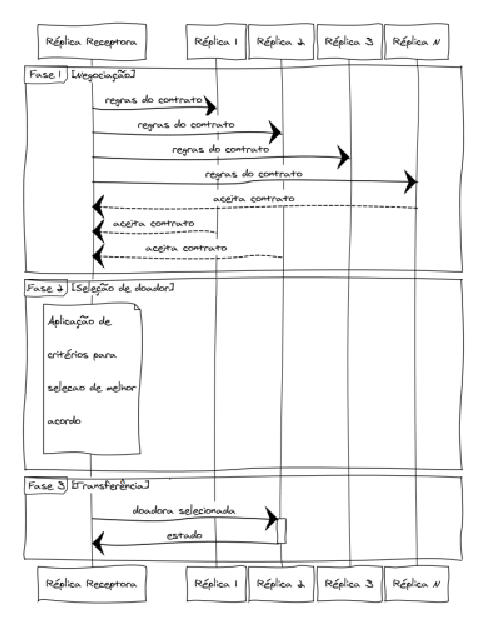
\includegraphics[width=11cm]{conteudo/capitulos/figuras/fases_protocolo.eps}
  \caption{Fases do protocolo de transferência de estado}
  \label{fig:fases_protocolo}
\end{figure}

Na Fase de Negociação, fase inicial, a réplica receptora estabelece as regras da
transferência de estado através da mensagem \classname{PolicyMessage}. Por exemplo,
supomos que, independente do motivo, uma réplica $r$ deseje receber um estado a partir da
instância de consenso $240$. Então, $r$ inicia a negociação de estado difundindo a
mensagem contratual. As réplicas que recebem essa mensagem de solicitação de negociação de
estado são solidárias e tentam atender essa requisição. Elas avaliam as exigências
contidas na mensagem e, caso estejam de acordo, enviam, somente para a replica receptora
(remetente do contrato), a mensagem \classname{DealMessage}. Essa proposta acordo, contém
informações referentes ao estado que a réplica doadora está oferecendo.

Caso a réplica receptora não receba nenhuma proposta de acordo após um tempo
pré-estabelecido, ela reinicia a Fase de Negociação até encontrar uma réplica doadora.
Podemos nos beneficiar desse \emph{loop} inicial que se encontra a réplica receptora para
criarmos diferentes políticas contratuais para transferência de estado. Nessa versão
proposta de Treplica, supomos configurações de duas politicas: uma mais agressiva e outra
mais ingênua. Lembrando que todas as políticas devem fornecer qual é a instância de
consenso pretendida.

\begin{itemize}
  \item Somente réplicas leitoras: essa política é mais restritiva, busca um acordo com
    uma réplica leitora \footnote{Réplicas leitoras são aquelas onde apenas os agentes
    proponente e aprendiz estão em execução. Elas não assumem um papel fundamental na
    execução de Paxos. Trataremos réplicas leitoras na \autoref{sec:replicas_leitoras}}.
    Acordos com réplica leitoras são preferíveis devido à restrição de sincronia exigida
    pelo protocolo. Dessa forma, essa política tenta minimizar possíveis impactos na
    computação de Paxos.
  \item Qualquer réplica: essa política é a menos restritiva possível, busca um acordo
    independente da configuração da réplica.
\end{itemize}

Devemos ter cuidado ao eleger uma réplica votante como réplica doadora, pois podemos gerar
impacto direto no desempenho da aplicação. A réplica doadora não participará da eleição de
um novo estado durante o período que está transmitindo seu estado (congelamento do estado
para garantia de consistência). Lembrando que, no algoritmo Paxos, a partir do momento em
que a maioria dos receptores concordam com a alteração do estado, mais cedo ou mais tarde
todas as réplicas chegarão ao mesmo estado. A partir do momento que retiramos
temporariamente da computação uma réplica votante, a probabilidade de atingir consenso
pela maioria diminui, podendo até impossibilitar o progresso do algoritmo.

O protocolo progride quando a réplica receptora possui propostas de acordo. Quando essa
condição é alcançada, ela inicia a Fase de Seleção de Doadora. Fase que executa um
algoritmo simples capaz de eleger a réplica que propôs o melhor acordo. Somente a partir
do momento que o algoritmo estabelece uma réplica doadora a Fase de Transferência inicia.
Para a execução dessa fase, os seguintes aspectos de Treplica foram considerados: (1) o
estado de uma aplicação pode ser tão grande quanto a capacidade de memória de uma réplica;
(2) todas as mensagens são trocadas utilizando o protocolo UDP.

Optamos então pela utilização do protocolo TCP para transferência de estado cobiçando
maior vazão dos dados nessa operação \cite{abdellatif04}. Somente o estado é enviado via
TCP, todas as outras mensagens pertencentes ao protocolo utilizam comunicação UDP, nativa
de Treplica. Sendo assim, a réplica receptora abre um \emph{socket} TCP e envia a mensagem
\classname{GETMessage} para a réplica doadora com o endereço do \emph{socket} TCP
recentemente aberto. Por sua vez, a réplica doadora bloqueia suas atividades e estabelece
a conexão TCP com a réplica leitora. Finalmente a transferência de estado é executada.

Assim que a operação é concluída, a conexão TCP entre as réplicas é finalizada. A réplica
doadora volta para computação e a réplica leitora começa a processar as requisições
encaminhadas pelos seus clientes. Estabelecemos um \emph{timeout} para evitar bloqueios
indevidos por falha em alguma das réplicas envolvidas na transação. Caso todas as etapas
do protocolo não sejam concluídas em no máximo 10 segundos, a negociação de estado é
reiniciada até que se obtenha êxito. A \autoref{fig:protocolo} ilustra o funcionamento do
protocolo com suas respectivas trocas de mensagens.

\begin{figure}[ht]
  \centering
  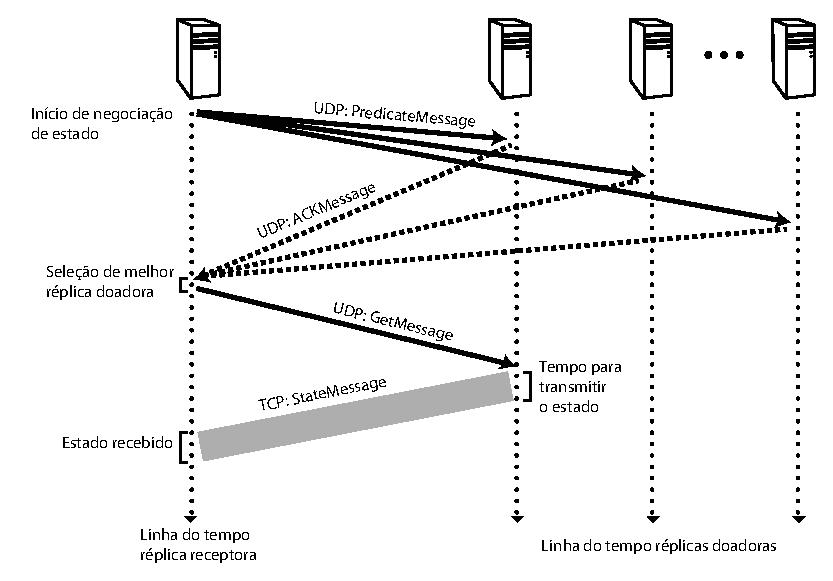
\includegraphics[width=11cm]{conteudo/capitulos/figuras/transferencia_estado.eps}
  \caption{Protocolo de transferência de estado}
  \label{fig:protocolo}
\end{figure}

\subsubsection{Componentes alterados}

O protocolo de transferência de estados possui quatro mensagens que são representadas
pelas classes \classname{PolicyMessage}, \classname{DealMessage}, \classname{GetMessage} e
\classname{StateMessage}. Todas essas classes implementam a interface de marcação
\classname{StateTransferMessage}, possibilitando assim, distinguir as mensagens do
protocolo das mensagens de Paxos.

Todas as mensagens do protocolo são roteadas no \emph{main loop} de cada réplica para a
classe \classname{Diplomat}, responsável pelo tratamento dessas mensagens, independente da
configuração existente na réplica.

\subsubsubsection{PolicyMessage}

A classe \classname{PolicyMessage} é a primeira mensagem do protocolo para transferência
de estado. Essa classe além de sinalizar para as outras réplicas do grupo que existe uma
réplica interessada em receber um estado, contém todas as informações sobre o estado
pretendido pela réplica receptora.

Os dados contratuais são abstraídos pela classe \classname{Policy}. Essa classe por sua
vez, contém o número da instância de consenso desejado (informação mínima para proposta de
um acordo) e uma lista de regras qualificadoras, que uma réplica deve atender para ser uma
doadora.

\subsubsubsection{DealMessage}

A classe \classname{DealMessage} também pertence ao grupo de mensagens trocadas pelo
protocolo de transferência. Essa classe abstrai uma proposta de acordo. Ela é uma
sinalização para a réplica receptora, informa a existência de uma réplica disposta a dor
seu estado (réplica doadora está em conformidade com a política estabelecida pela réplica
receptora). Quanto mais mensagens propondo acordo de transferência uma réplica receptora
receber, menos restritivas são suas políticas, potencializando a seleção de uma réplica
votante.

\subsubsubsection{GetMessage}

A classe \classname{GetMessage} é a abstração da mensagem de pedido de estado enviada
somente para a réplica doadora. As informações do endereço para envio do estado (através
de \emph{socket} TCP) é extraído dessa mensagem.

\subsubsubsection{StateMessage}

A classe \classname{StateMessage} é a abstração do estado enviado da réplica doadora para
a réplica receptora. Essa classe possuí como atributos o número da instância de consenso
(último decreto que causou alteração no estado) e um estado no formato
\classname{java.io.Serializable}. Definimos essa classe como uma cópia instantânea, tirada
no no período que a réplica está bloqueada para alterações.

A partir do conteúdo armazenado por \classname{StateMessage}, qualquer réplica que possuí
uma visão de estado menor \footnote{Podemos supor comparações de estados através da última
instância de consenso, já que o mesmo é um limiar crescente \cite{vieira-10b}.} pode se
beneficiar da substituição de seu estado local corrente (desatualizado) por um mais atual,
com potencial chance de ser o estado corrente compartilhado pela maioria grupo, conforme
especificação de Paxos.

\subsubsubsection{Diplomat}

A classe \classname{Diplomat} é responsável por implementar o tratamento das mensagens do
protocolo de trasferência. Toda réplica, independente da configuração, possui uma
instância da classe \classname{Diplomat} para representar seus interesses frente outras
réplicas. A abstração desse componente foi inspirada nas funções de diplomacia (ciência e
arte referentes às relações entre Estados \cite{aurelio}) exercidas por um Diplomata no
modelo atual de relação entre nações \footnote{Segundo \citeonline{aurelio}, diplomata é
um funcionário que representa um governo junto de outro governo.}.

O Diplomata adéqua suas funções de trabalho conforme o estado corrente da replica. Em uma
réplica receptora, está habilitado as funções responsáveis por obter um novo estado:
criação de política, seleção de réplica doadora e abertura de \emph{socket} TCP. Por outro
lado, em uma réplica doadora as funções para ceder o estado é que estão habilitadas:
análise de aderência a política de transferência, bloqueio de alterações de estado e o
envio de estado.

Para seleção da melhor proposta de transferência de estado, o Diplomata armazena em
memória todas as propostas recebidas e após o estouro de um \emph{timeout} estabelecido, a
seleção é realizada. Consideramos como melhor proposta de estado aquela que possui maior
instância de consenso. Em caso de eventuais erros e/ou \emph{timeouts} as propostas são
removidas da memória para evitar conflitos com as futuras propostas de acordo, que serão
recebidas devido atuação do mecanismo de reinicialização.

\subsubsection{Política de Reconfiguração}

Identificamos dois potenciais pontos que se beneficiariam da utilização do protocolo de
transferência de estado: (1) expansão do aglomerado e (2) recuperação de erros. Para a
construção desse trabalho, focamos na aplicação do protocolo na expansão do aglomerado,
conforme ilustra a \autoref{fig:inclusao}. Supomos alguns aspecto para serem considerados:

\begin{itemize}
  \item O estado da nova réplica que deseja se juntar ao aglomerado está defasado com
    relação ao estado das réplicas que já participam do grupo. É imprescindível que essa
    defasagem seja suprimida.
  \item A operação para igualar o estado da nova réplica com o estado compartilhado pelo
    grupo deve ser consistente.
  \item O impacto gerado para o processamento do aglomerado deve ser mínimo.
\end{itemize}

Para justificar a inclusão de uma nova réplica, obrigatoriamente é preciso geração de
benefícios para o processamento em grupo, caso contrário estamos executando operações sem
serventia com potencial para saturar o sistema.

\begin{figure}[ht]
  \centering
  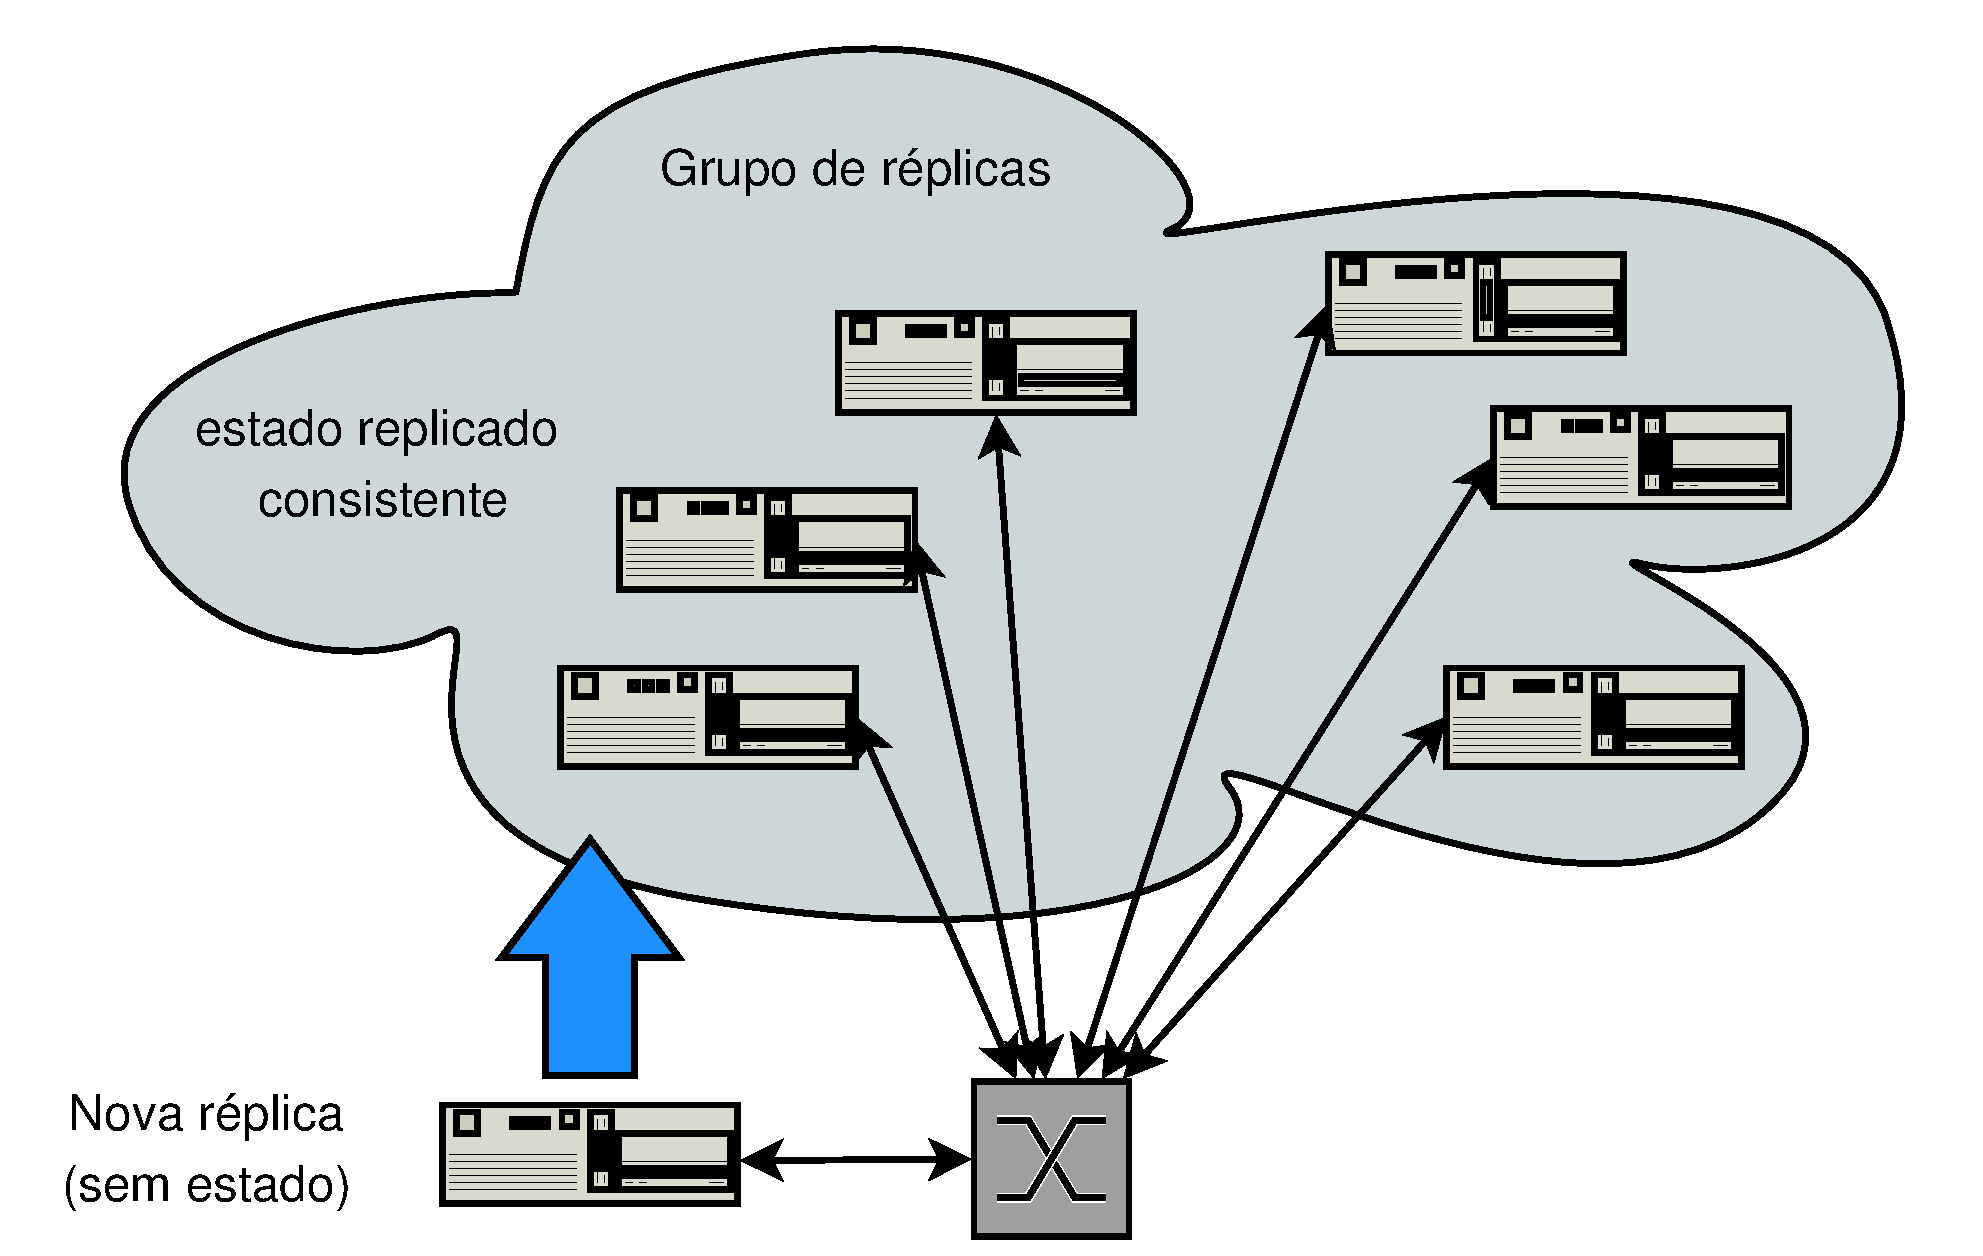
\includegraphics[width=11cm]{conteudo/capitulos/figuras/inclusao_replica_cluster.eps}
  \caption{Inclusão de réplica}
  \label{fig:inclusao}
\end{figure}

\citeonline{lamport10} apresenta em seu trabalho um mecanismo para reconfiguração que pode
ser aplicados em réplicas votantes, através da criação de diferentes formações de grupos
representados por visões, controladas por um identificador sequencial. Como estamos
trabalhando no modelo computacional assíncrono com falha-e-recuperação, a aplicação dessa
proposta é complexa. Se analisarmos um instante no tempo, diferentes visões poderão estar
sendo executadas simultaneamente com a visão corrente (visão com maior identificador). O
gerenciamento dessas visões e a formação de diferentes grupos não é uma tarefa trivial.

Investimos nosso esforço na construção de um mecanismo que tenta fugir da complexidade do
mecanismo de visões proposto por \citeonline{lamport10}, consequentemente evitamos
reconfigurações em réplicas votantes e focamos na criação e remoção de réplicas leitoras.
A motivação por trás da criação de réplicas leitoras é permitir que o sistema reaja de
forma autônoma a picos de carga sem comprometer o desempenho do mesmo. No entanto, sem uma
política cuidadosa de reconfiguração corre-se o risco de gastar muitos dos recursos do
sistema no próprio processo de reconfiguração, anulando quaisquer ganhos advindos do
acréscimo de novas réplicas leitoras.

A política de reconfiguração deve, desta forma, ser um equilíbrio entre o custo de se
instanciar uma nova réplica leitora e os ganhos de desempenho a serem auferidos após esta
instanciação. O trabalho de especificação de parâmetros para esta política ainda está em
seu estágio inicial, dependendo de estudos mais aprofundados para caracterizar os custos
envolvidos.

\subsection{Paxos com Réplicas Leitoras}\label{sec:replicas_leitoras}

A ideia principal da abordagem proposta é utilizar réplicas que não participem do processo
de decisão de instâncias de consenso. Isso é feito com a adoção de \emph{réplicas
leitoras}, que são réplicas onde apenas parte dos agentes do algoritmo Paxos estão
executando. Para maior clareza de exposição, quando necessário, chamaremos as réplicas
contendo todos os agentes ativos de \emph{réplicas votantes}. Para suportar a adaptação
elástica a novos perfis de desempenho, desenvolvemos um mecanismo para o
\emph{provisionamento de réplicas} e uma \emph{política de reconfiguração}.

\subsubsection{Réplicas Leitoras}

Réplicas leitoras são réplicas onde apenas os agentes proponente e aprendiz estão
executando. Dessa forma, do ponto de vista do conjunto de processos que implementam o
algoritmo Paxos, uma réplica leitora é capaz apenas de propor operações a serem aplicadas
no estado replicado e de aprender operações decididas pelo conjunto de receptores. Do
ponto de vista do cliente da aplicação replicada um réplica leitora se comporta como uma
réplica votante: ela atende requisições de qualquer tipo garantindo a execução atômica das
mesmas.

As réplicas leitoras não assumem um papel fundamental na execução do algoritmo Paxos, no
entanto elas se integram de forma consistente com a operação das réplicas votantes por
meio de suas funções fundamentais: propor e aprender requisições de escrita. As réplicas
leitoras propõem novas requisições a serem executadas em nome de seus clientes através de
seu agente proponente. O proponente encaminha a operação ao coordenador que por sua vez
decide, em conjunto com os receptores, a ordem da mesma através de uma rodada de Paxos,
como descrito no \autoref{cap1:replicacao_ativa_paxos}. Uma vez que a decisão é alcançada,
a mesma é difundida para o resto do sistema. Nesse momento o agente aprendiz da réplica
leitora toma conhecimento da decisão e atualiza o seu estado interno, sem a participação
ativa do coordenador ou de qualquer receptor.

Tanto o processo de proposta quanto o de aprendizado executado por uma réplica leitora
devem usar as mesmas estratégias de implementação das réplicas votantes. Na verdade, em
nossa implementação usando Treplica, as réplicas leitoras foram construídas a partir da
separação modular dos agentes que implementam Paxos. Dessa forma, reutilizamos os mesmos
componentes e por consequência essas réplicas são capazes de detectar e reenviar propostas
perdidas, detectar e corrigir lacunas na sequência de instâncias de consenso, fazer
controle de fluxo e de congestionamento, entre outras operações fundamentais para uma
operação eficiente de Paxos \cite{vieira-tr10b}.

Uma consequência importante do uso de réplicas leitoras é que essas réplicas,
consistentemente com as funções que elas assumem no algoritmo Paxos, não precisam de
memória persistente para sua operação. Isso se deve ao fato de que elas não executam as
Fases 1 e 2 do algoritmo. Porém, pode ser interessante que essas réplicas registrem a
proposta decidida de forma a não precisar realizar uma recuperação completa em caso de
falha. Na nossa proposta de réplicas leitoras decidimos não fazer esse registro de forma a
remover completamente a escrita em memória persistente do caminho crítico de execução. É
interessante observar que a escrita eliminada ocorre somente quando a réplica leitora
atualiza o seu estado de acordo com as propostas decididas pelos receptores das réplicas
votantes. Dessa forma, as réplicas leitoras conseguem manter seu estado atualizado com as
réplicas votantes com um custo mínimo. Elas também são capazes de processar requisições de
escrita com um custo similar àquele gerado pelas réplicas votantes ao executar as mesmas
requisições. Podemos argumentar que esse custo é menor, na medida que as réplicas leitoras
aliviam as réplicas votantes do custo de manter as conexões abertas com os clientes.

Utilizando réplicas leitoras, podemos formar grupos de réplicas com diferentes graus de
uso de memória persistente \cite{aguilera00}. Uma configuração simples seria mesclar
réplicas votantes e leitoras formando um conjunto híbrido de réplicas transparente para o
cliente, conforme ilustra a \autoref{fig:configuracao_replicas_leitoras} (a). É concebível
ainda uma configuração onde as réplicas votantes não entram em contato com os clientes,
sendo essa operação completamente delegada às replicas leitoras, configuração ilustrada
pela \autoref{fig:configuracao_replicas_leitoras} (b).

\begin{figure}[ht]
  \begin{center}
    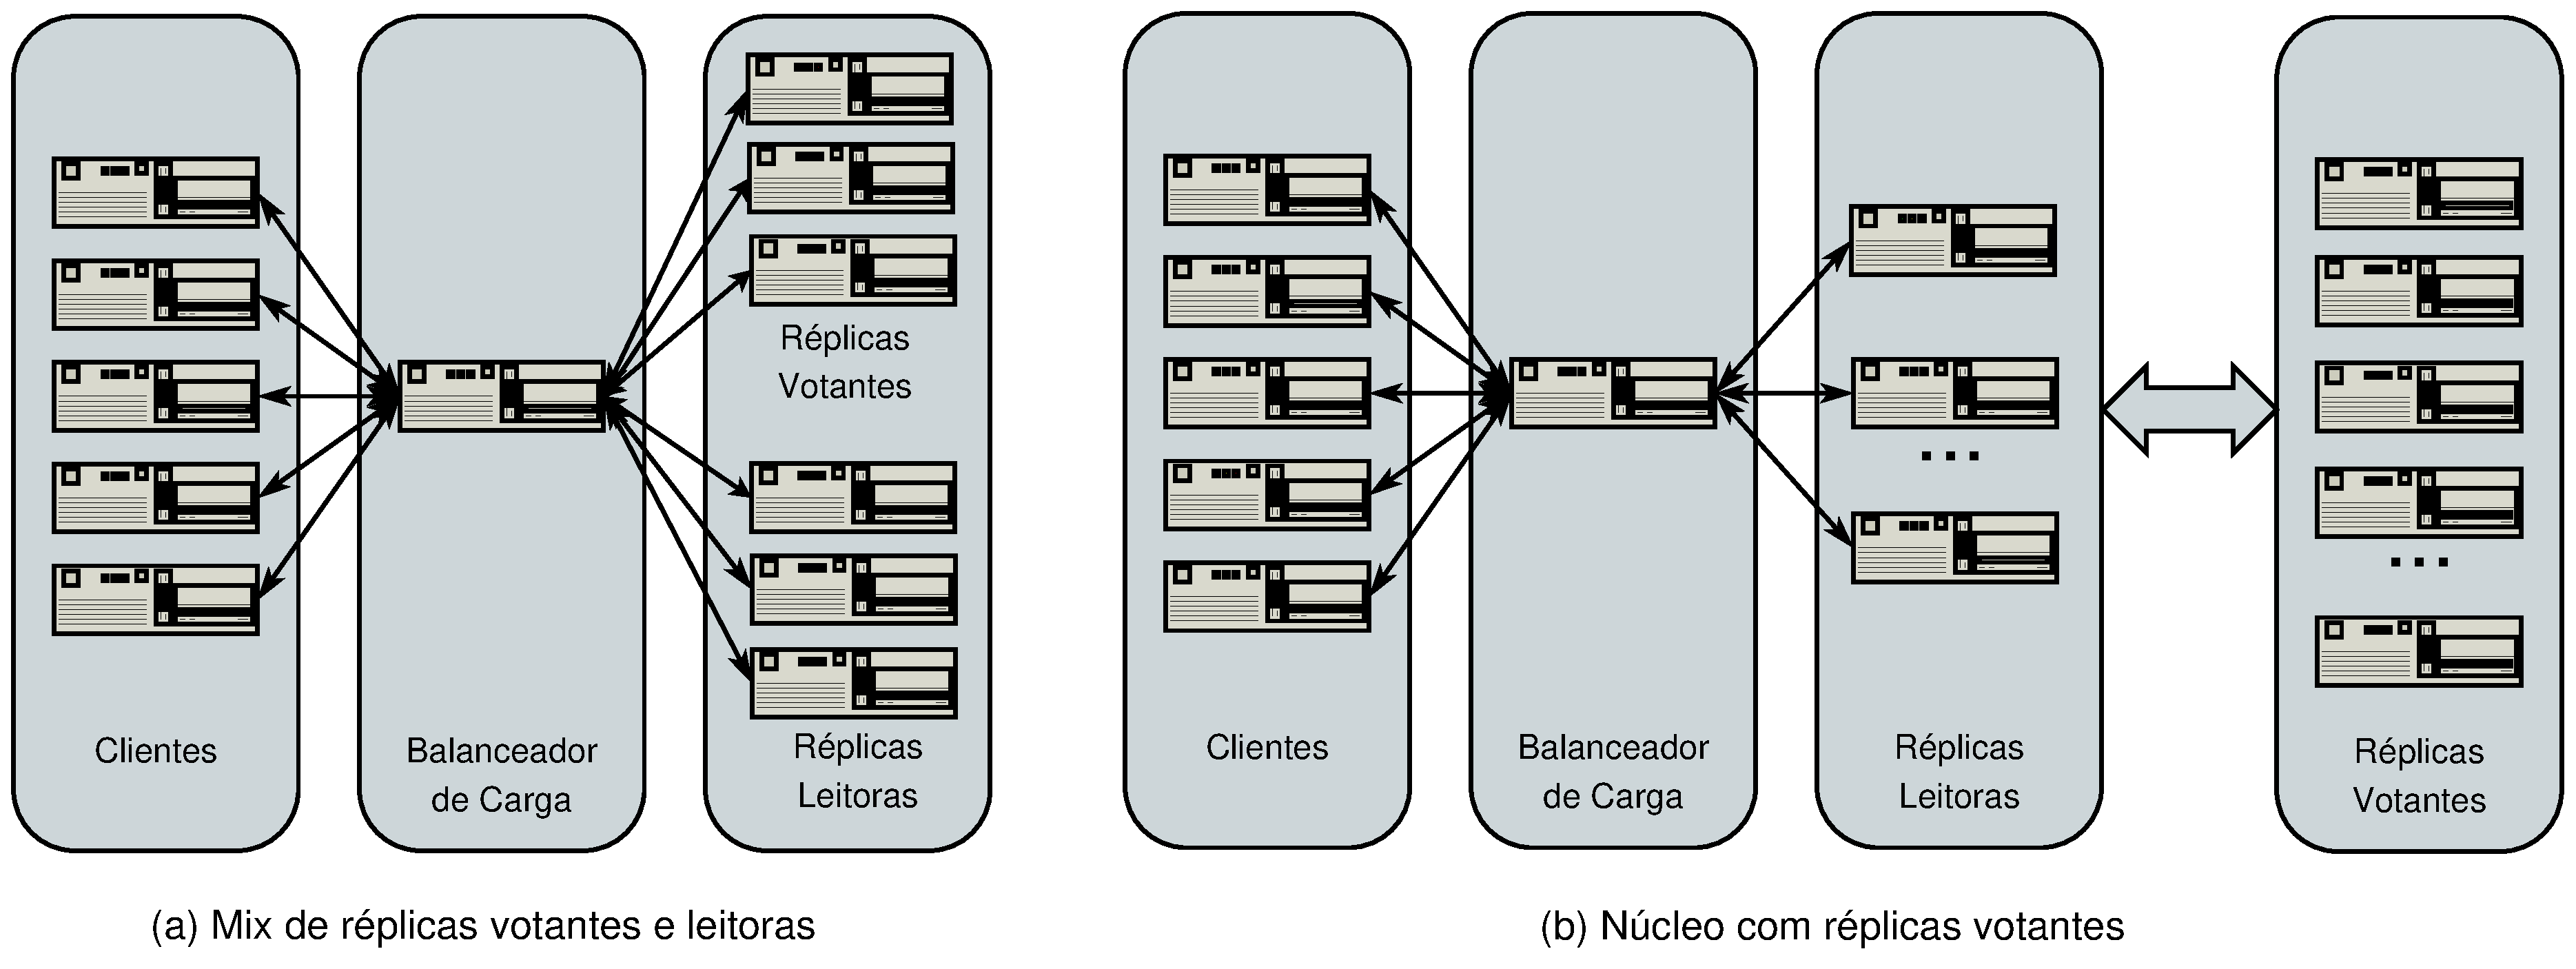
\includegraphics[width=16cm]{conteudo/capitulos/figuras/configuracao_replicas_leitoras.eps}
  \end{center}
  \caption{Configuração de Paxos com réplicas votantes e leitoras}
  \label{fig:configuracao_replicas_leitoras}
\end{figure}

As réplicas leitoras funcionam então como uma espécie de cache \emph{write-through}
distribuído. O estado replicado na memória destas réplicas permite atender diretamente as
requisições de leitura dos clientes, enquanto as requisições de escrita são repassadas ao
receptores. Podemos ver claramente que a taxa de acerto desse cache está diretamente
ligada à proporção de operações de leitura geradas pelos clientes e que a vazão de
operações de leitura tem o potencial de crescer linearmente com o número de réplicas
leitoras disponíveis.

\subsubsection{Componentes alterados}

Antes de detalharmos as alterações realizadas, vamos recapitular de forma resumida a
iteração entre os agentes de Paxos: proponentes enviam a sua proposta para o coordenador
que tenta alcançar consenso sobre a proposta em uma rodada, sendo que cada proposta
corresponde a uma ou mais requisições de escrita da aplicação sendo replicada.

Anteriormente, era possível uma única configuração de réplicas que empregava todos os
agentes de Paxos utilizando memória persistente. A nova funcionalidade de réplicas
leitoras foi implementada através de uma segregação modular dos agentes utilizados por uma
réplica votante:

\begin{itemize}
  \item Proponente: agente capaz de propor valores;
  \item Receptor: agente que vota em uma única proposta por rodada;
  \item Aprendiz: agente que aprende a decisão de consenso;
  \item Coordenador: agente responsável por garantir o funcionamento do algoritmo a cada
    rodada de consenso executada.
\end{itemize}

A classe denominada \classname{PaxosPersistentQueue} é responsável por implementar o
agrupamento de todos esses agentes, caracterizando assim uma réplica votante. Podemos
definir, do ponto de vista de uma Máquina Virtual Java (JVM), que uam réplica votante
possui como uma das suas \emph{threads} ativas o \emph{main loop} da classe
\classname{PaxosPersistentQueue}. Em contra partida, uma réplica leitora, executa o
\emph{main loop} da classe \classname{PaxosReadonlyQueue}. Essa classe, implementa somente
a agregação dos agentes proponente e aprendiz, sem a utilização de memória persistente.
Detalharemos nas próximas seções a implementação proposta para esse componente.

\subsubsubsection{PaxosReadonlyQueue}

A classe \classname{PaxosReadonlyQueue} foi criada para fornecer o mesmo comportamento da
classe \classname{PaxosPersistenteQueue}: disponibilizar uma fila que será utilizada pelo
protocolo Paxos. No entanto, as operações suportadas por \classname{PaxosReadonlyQueue}
não as mesmas. Do ponto de vista do processamento de mensagens postadas na fila, as
seguintes propriedades foram supostas para caracterizar uma réplica leitora:

\begin{itemize}
  \item Abdicar liderança: todas as mensagens relacionadas a eleição de líder não são
    processadas, logo é eliminada qualquer possibilidade de uma réplica leitora se tornar
    coordenadora de uma rodada de Paxos.
  \item Inelegível ao voto: mensagens relacionadas a votação de uma proposta são
    ignoradas. Dessa forma, réplicas leitoras não participam do processo de decisão de
    consenso e não são essenciais para o progresso do algoritmo Paxos.
  \item Aprendizado: todas as mensagens endereçadas ao componente \classname{Learner} são
    processadas pela fila. Consequentemente, os mecanismos descobrir qual foi o consenso
    de uma determinada rodada são habilitados.
\end{itemize}

O principal objetivo dessa classe é participar das operações que não exigem dados
persistentes para garantir correção do algoritmo, oferecendo instâncias capazes de atuar
parcialmente nas fases de Paxos. Do ponto de vista do cliente da aplicação um réplica
leitora se comporta como uma réplica votante: ela atende requisições de qualquer tipo
garantindo a execução atômica das mesmas. Sendo assim, as seguintes premissas não podem
ser violadas:

\begin{itemize}
  \item Mensagens quem alteram o estado (escrita): são resolvidas pelo aglomerado de
    réplicas orquestrado pelo protocolo Paxos, porém réplicas que não possuem grau de
    memória persistente não participam da decisão de consenso.
  \item Mensagens que não alteram estado (leitura): são resolvidas localmente independente
    do grau de memória da réplica.
\end{itemize}

Do ponto de vista de uma réplica votante, não é possível distinguir se a proposta é
oriunda de uma réplica votante ou leitora. O mecanismo para configuração do grau de
memória de uma réplica em Treplica atua de forma transparente junto com protocolo Paxos,
respeitando a forte premissa: o número de réplicas leitoras nunca deve afetar o número de
réplicas votantes. Sendo assim, podemos afirmar que o progresso e a correção do algoritmo
não são violados.

Réplicas oferecem um poder de manobra para aliviar a carga de processamento das réplicas
votantes com relação a mensagens de leituras, podendo ser configuradas de tal forma que
nenhuma mensagem de leitura seja processada por uma réplica votante. Avaliar e propor
soluções para configuração do conjunto de réplicas não faz parte do escopo desse trabalho.

\subsubsubsection{WeakSecretary}

A classe \classname{WeakSecretary} apresenta uma abstração de I/O sem persistência de
dados em disco. Esse componente é uma versão leve da classe \classname{Secretary}, ela é
utilizada pelos agentes de Paxos para enviar mensagens pela rede, através do intermédio do
componente \classname{Transport}. Essa classe foi projetada para trabalhar com dados
somente em memória, dessa forma todos os dados computados são perdidos na presença de
defeitos na réplica. No entanto, na ausência de falhas nos beneficiamos da eliminação de
uma operação custosa relacionada com I/O em disco.

\classname{WeakSecretary} também é responsável por lidar com o componente
\classname{Ledger} e com a fila de objetos utilizada para entregar mensagens para a camada
da aplicação. A principal razão para a criação dessa abstração em Treplica foi eliminar a
operação de persistência em disco, gerando um componente volátil, capaz de oferecer as
operações essenciais para o progresso do algoritmo sem o ônus da escrita em disco.

\subsubsection{Provisionamento de Réplicas Leitoras}

É possível utilizar os mecanismos tradicionais de Treplica para provisionar uma nova
réplica leitora. Em resumo, uma réplica que se integra ao sistema pela primeira vez ou
após uma falha demorada deve recuperar o seu estado. Esse processo acontece através de um
mecanismo de preenchimento de lacunas, que observa que não pode executar novas requisições
de escrita sem antes executar as requisições anteriores \cite{vieira-tr10b}. Esse
procedimento é voltado para reparar pequenas interrupções e não a recuperação do estado
completo de uma réplica. Em particular, no caso de uma réplica leitora sem estado
persistente, o tamanho dessa recuperação pode ser muito grande em termos do número de
\emph{requisições} a serem reexecutadas, pois ela sempre parte do estado inicial vazio.

Foi necessário então criar um procedimento de provisionamento de réplicas, de forma a
permitir o rápido início de uma réplica leitora. Esse mecanismo não é necessariamente
exclusivo de réplicas leitoras e pode ser aplicado a réplicas normais. Porém, neste
primeiro momento, ele tira proveito do fato dessas réplicas não terem memória persistente.
Em particular, a adição ou remoção de uma réplica leitora não altera o número de
receptores executando o algoritmo, não havendo necessidade de se realizar um
reconfiguração custosa \cite{lamport10}.

\subsection{Transferência de estado para recuperação de falhas}

Treplica possui outro potencial candidato para empregar o protocolo de transferência: o
componente detector lacunas na sequência de instâncias de consenso. Lacunas podem surgir
por diferentes motivos: falha-e-recuperação na réplica, perda de mensagens ou ainda
réplicas com grandes diferenças de capacidade de processamento. Para preencher lacunas
detectadas, o componente solicita retransmissão da instância de consenso em uma
determinada rodada. É perceptível que na presença de grandes lacunas essa abordagem
exigirá uma longa sequência de retransmissões.

Para exemplificar o potencial problema do detector de lacunas, vamos supor que a aplicação
$x$ está passando por um grande pico de processamento (\emph{flash crowds}) e que a
réplica $r$ possui uma grande lacuna. O mecanismo detector de lacunas solicitará
retransmissão das instâncias de consenso não conhecidas por ele, aumentando a concorrência
no meio compartilhado pelas réplicas: a rede. Como solução alternativa, podemos utilizar o
mecanismo de transferência, para concentrar em uma única mensagem, o estado resultante das
aplicações das instâncias de consenso. Dessa forma, o novo mecanismo suposto para detectar
lacunas tem capacidade de:

\begin{itemize}
  \item Retransmissão de instância de consenso: utilizado para preencher pequenas lacunas
    na sequência de consenso.
  \item Protocolo de transferência de estado: utilizado para preencher grandes lacunas,
    onde retransmissão tem potencial perda de desempenho.
\end{itemize}

